\documentclass{minimal}
\usepackage{graphicx,color}
\usepackage[utf8]{inputenc}
\usepackage[papersize={418.00bp,314.00bp},text={418.00bp,314.00bp}]{geometry}
\begin{document}
\centering
% Title: gl2ps_renderer figure
% Creator: GL2PS 1.4.2, (C) 1999-2020 C. Geuzaine
% For: Octave
% CreationDate: Mon Dec 12 16:54:16 2022
\setlength{\unitlength}{1pt}
\begin{picture}(0,0)
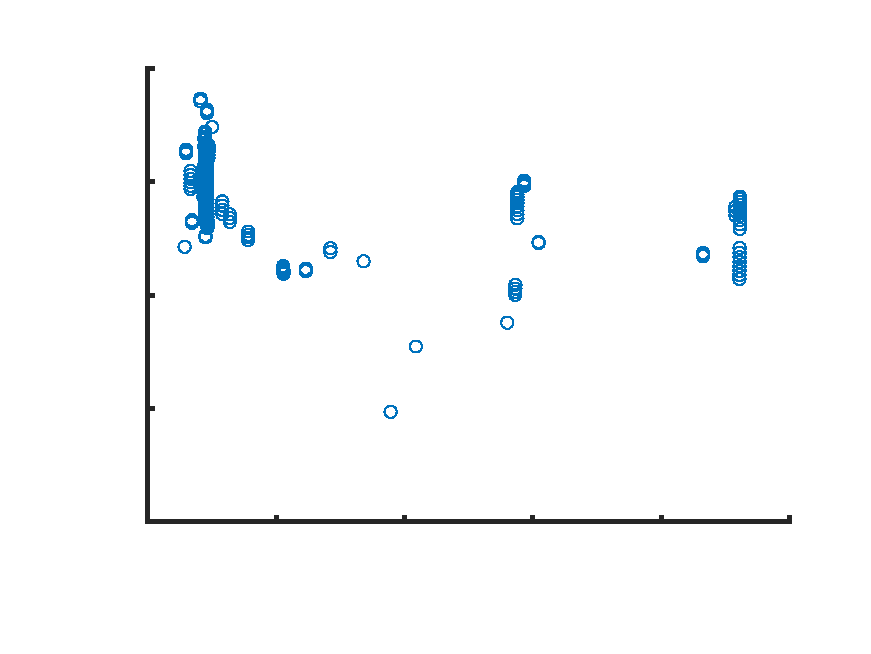
\includegraphics[scale=1]{DoubleKapitzaPoincare-inc}
\end{picture}%
\begin{picture}(418,314)(0,0)
\fontsize{22}{0}\selectfont\put(70.9982,46.956){\makebox(0,0)[t]{\textcolor[rgb]{0.15,0.15,0.15}{{-50}}}}
\fontsize{22}{0}\selectfont\put(132.588,46.956){\makebox(0,0)[t]{\textcolor[rgb]{0.15,0.15,0.15}{{-40}}}}
\fontsize{22}{0}\selectfont\put(194.177,46.956){\makebox(0,0)[t]{\textcolor[rgb]{0.15,0.15,0.15}{{-30}}}}
\fontsize{22}{0}\selectfont\put(255.767,46.956){\makebox(0,0)[t]{\textcolor[rgb]{0.15,0.15,0.15}{{-20}}}}
\fontsize{22}{0}\selectfont\put(317.357,46.956){\makebox(0,0)[t]{\textcolor[rgb]{0.15,0.15,0.15}{{-10}}}}
\fontsize{22}{0}\selectfont\put(378.946,46.956){\makebox(0,0)[t]{\textcolor[rgb]{0.15,0.15,0.15}{{0}}}}
\fontsize{22}{0}\selectfont\put(60,63.4239){\makebox(0,0)[r]{\textcolor[rgb]{0.15,0.15,0.15}{{-15}}}}
\fontsize{22}{0}\selectfont\put(60,117.818){\makebox(0,0)[r]{\textcolor[rgb]{0.15,0.15,0.15}{{-10}}}}
\fontsize{22}{0}\selectfont\put(60,172.212){\makebox(0,0)[r]{\textcolor[rgb]{0.15,0.15,0.15}{{-5}}}}
\fontsize{22}{0}\selectfont\put(60,226.606){\makebox(0,0)[r]{\textcolor[rgb]{0.15,0.15,0.15}{{0}}}}
\fontsize{22}{0}\selectfont\put(60,281){\makebox(0,0)[r]{\textcolor[rgb]{0.15,0.15,0.15}{{5}}}}
\fontsize{24}{0}\selectfont\put(224.972,24.956){\makebox(0,0)[t]{\textcolor[rgb]{0.15,0.15,0.15}{{$\theta_2/(2 \pi)$}}}}
\fontsize{24}{0}\selectfont\put(24,172.212){\rotatebox{90}{\makebox(0,0)[b]{\textcolor[rgb]{0.15,0.15,0.15}{{$\omega_2$}}}}}
\fontsize{24}{0}\selectfont\put(224.972,291){\makebox(0,0)[b]{\textcolor[rgb]{0,0,0}{{Poincaré Section at $\theta_1 = 0$}}}}
\end{picture}
\end{document}
